\documentclass[11pt,a4paper]{article}

%========== PACKAGES ==========%

\usepackage{a4wide} 			% save some rainforests
\usepackage{amsmath,amssymb}	% for mathematical notation
\usepackage[english]{babel}		% language definition
\usepackage{color}				% to make syntax pretty
\usepackage{enumerate}			% roman enumeration
\usepackage{fancyref}			% fancy references
\usepackage{float}				% for precise placement
\usepackage{graphicx}			% importing graphics
\usepackage{listings}			% code listings
\usepackage[utf8]{inputenc} 	% can we has UTF-8, plox
\usepackage{multicol} 			% for column layout
\usepackage{tikz} 				% pretty drawings

\usetikzlibrary{automata,arrows,positioning}	% make things easier

%========== DEFINITIONS ==========%

\definecolor{comment}{rgb}		{0.38, 0.62, 0.38}
\definecolor{keyword}{rgb}		{0.10, 0.10, 0.81}
\definecolor{identifier}{rgb}	{0.00, 0.00, 0.00}
\definecolor{string}{rgb}		{0.50, 0.50, 0.50}

%========== SETTINGS ==========%

\lstset
{
	% general settings
	numbers=left,
	frame=single,
	basicstyle=\footnotesize\ttfamily,
	tabsize=2,
	% syntax highlighting
	commentstyle=\color{comment},
	keywordstyle=\color{keyword},
	identifierstyle=\color{identifier},
	stringstyle=\color{string},
}

%========== DECLARATIONS ==========%

\title
{
	{\large Individual Assignment 1}\\
	Compilers
}

\author
{
	Casper B. Hansen\\
	Department of Computer Science\\
	University of Copenhagen\\
	{\tt fvx507@alumni.ku.dk}
}

%========== DOCUMENT ==========%

\begin{document}

\clearpage
\maketitle

\section{DFA Minimisation}
Minimise the DFA given below, following the algorithm presented in the
lecture.
\begin{figure}[H]
	\center
	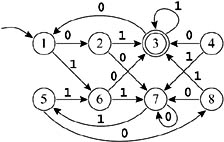
\includegraphics[scale=1.0]{figures/dfatominimise}
	\label{fig:dfa-to-minimise}
	\caption{Deterministic Finite Automaton}
\end{figure}
Using the algorithm presented in the lecture, we have that only one state
$F = \{s_3\}$ is considered {\it accepting}, as such we need not consider
it for equivalence, the group for consideration is therefore simply $S{\ }
\backslash F = \{s_1,s_2,s_4,s_5,s_6,s_7,s_8\}$.

We now list the individual states with their respective transitions
\begin{align*}
	s_1 = 
	\begin{cases}
		s_2 &\mbox{iff. 0}\\
		s_6 &\mbox{iff. 1}
	\end{cases}
	\qquad
	s_2 =
	\begin{cases}
		s_7 &\mbox{iff. 0}\\
		s_3 &\mbox{iff. 1}
	\end{cases}
	\qquad
	s_4 =
	\begin{cases}
		s_3 &\mbox{iff. 0}\\
		s_7 &\mbox{iff. 1}
	\end{cases}
	s_5 = 
	\begin{cases}
		s_8 &\mbox{iff. 0}\\
		s_6 &\mbox{iff. 1}
	\end{cases}
\end{align*}
\begin{align*}
	s_6 =
	\begin{cases}
		s_3 &\mbox{iff. 0}\\
		s_7 &\mbox{iff. 1}
	\end{cases}
	\qquad
	s_7 =
	\begin{cases}
		s_7 &\mbox{iff. 0}\\
		s_5 &\mbox{iff. 1}
	\end{cases}
	\qquad
	s_8 =
	\begin{cases}
		s_7 &\mbox{iff. 0}\\
		s_3 &\mbox{iff. 1}
	\end{cases}
\end{align*}
\newpage\noindent
From this, we see that $s_2 \sim s_8$ and $s_4 \sim s_6$. This gets rid of two
of the states; namely, $s_4$ and $s_8$. Substituting the transitions leading
to these for the equivalent ones; namely, $s_6$ and $s_2$, respectively, we
have that
\begin{align*}
	s_1 = 
	\begin{cases}
		s_2 &\mbox{iff. 0}\\
		s_4 &\mbox{iff. 1}
	\end{cases}
	\quad
	s_2 =
	\begin{cases}
		s_7 &\mbox{iff. 0}\\
		s_3 &\mbox{iff. 1}
	\end{cases}
	\quad
	s_4 =
	\begin{cases}
		s_3 &\mbox{iff. 0}\\
		s_7 &\mbox{iff. 1}
	\end{cases}
	\quad
	s_5 = 
	\begin{cases}
		s_2 &\mbox{iff. 0}\\
		s_4 &\mbox{iff. 1}
	\end{cases}
	\quad
	s_7 =
	\begin{cases}
		s_7 &\mbox{iff. 0}\\
		s_5 &\mbox{iff. 1}
	\end{cases}
\end{align*}
Yet again, we have that $s_1 \sim s_5$, and so we substitute this. We then
have that
\begin{align*}
	s_1 = 
	\begin{cases}
		s_2 &\mbox{iff. 0}\\
		s_4 &\mbox{iff. 1}
	\end{cases}
	\qquad
	s_2 =
	\begin{cases}
		s_7 &\mbox{iff. 0}\\
		s_3 &\mbox{iff. 1}
	\end{cases}
	\qquad
	s_4 =
	\begin{cases}
		s_3 &\mbox{iff. 0}\\
		s_7 &\mbox{iff. 1}
	\end{cases}
	\qquad
	s_7 =
	\begin{cases}
		s_7 &\mbox{iff. 0}\\
		s_1 &\mbox{iff. 1}
	\end{cases}
\end{align*}
And thus, we end up with the minimised DFA
\begin{figure}[H]
	\center
	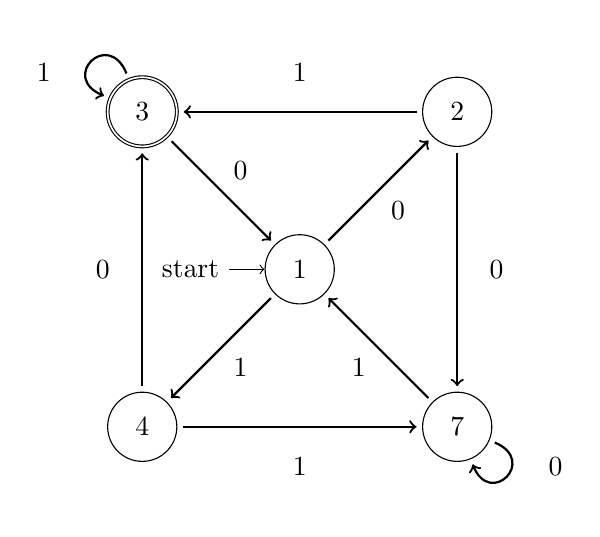
\begin{tikzpicture}
		[
			transform shape,
			scale=1.0,
			align=center,
			label/.style={draw=none,fill=none},
			arrow/.style={->, thick, shorten <=2pt, shorten >=2pt,}
		]

		% states
		\node[initial,state]		(s1) at (  0.0,  0.0 ) {$1$};
		\node[state]				(s2) at (  2.0,  2.0 ) {$2$};
		\node[state,accepting]		(s3) at ( -2.0,  2.0 ) {$3$};
		\node[state]				(s4) at ( -2.0, -2.0 ) {$4$};
		\node[state]				(s7) at (  2.0, -2.0 ) {$7$};

		% transition labels
		\node[label] (s1s2) at (  1.25,  0.75 ) {$0$};
		\node[label] (s1s4) at ( -0.75, -1.25 ) {$1$};

		\node[label] (s2s7) at (  2.50,  0.00 ) {$0$};
		\node[label] (s2s3) at (  0.00,  2.50 ) {$1$};

		\node[label] (s3s7) at ( -0.75,  1.25 ) {$0$};
		\node[label] (s3s3) at ( -3.25,  2.50 ) {$1$};

		\node[label] (s4s7) at ( -2.50,  0.00 ) {$0$};
		\node[label] (s4s3) at (  0.00, -2.50 ) {$1$};

		\node[label] (s7s7) at (  3.25, -2.50 ) {$0$};
		\node[label] (s7s1) at (  0.75, -1.25 ) {$1$};

		% transition paths
		\foreach \from/\to in
		{
			s1/s2, s1/s4,
			s2/s7, s2/s3,
			s3/s1, s7/s1,
			s4/s3, s4/s7}
		\draw[arrow] (\from) -> (\to);
		\draw[arrow] (s3) to [out=112.5,in=157.5,looseness=5] (s3);
		\draw[arrow] (s7) to [out=337.5,in=292.5,looseness=5] (s7);

	\end{tikzpicture}
	\label{fig:minimised-dfa}
	\caption{Minimised DFA}
\end{figure}

\newpage
\section{Backtracking Automaton}
Given the following regular expressions

\begin{multicols}{5}
	
	{\ }\vfill\columnbreak % dummy

	\centering
	\begin{itemize}
		\item[$\alpha_1$:] \verb/ab*/
	\end{itemize}

	\vfill
	\columnbreak

	\centering
	\begin{itemize}
		\item[$\alpha_2$:] \verb/a*b/
	\end{itemize}

	\vfill
	\columnbreak

	\centering
	\begin{itemize}
		\item[$\alpha_3$:] \verb/(ab)*c/
	\end{itemize}

	\vfill\columnbreak{\ } % dummy

\end{multicols}

\subsection*{a \mdseries Give an NFA for each expression (no particular
method required), and construct a combined NFA to recognise $L(\alpha_1)$,
$L(\alpha_2)$, and $L(\alpha_3)$.}
Following the rules given on the slides from the lecture, we get that
\begin{multicols}{3}

	\begin{figure}[H]
		\center
		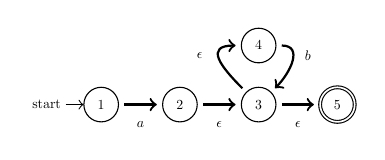
\begin{tikzpicture}
			[
				transform shape,
				scale=0.5,
				align=center,
				label/.style={draw=none,fill=none},
				arrow/.style={->, thick, shorten <=2pt, shorten >=2pt,}
			]

			% states
			\node[initial,state] (s1) at (  0.0,  0.0 ) {$1$};
			\node[state] (s2) at (  2.0,  0.0 ) {$2$};
			\node[state] (s3) at (  4.0,  0.0 ) {$3$};
			\node[state] (s4) at (  4.0,  1.5 ) {$4$};
			\node[state,accepting] (s5) at (  6.0,  0.0 ) {$5$};

			% transition labels
			\node[label] (s1s2) at (  1.0 , -0.5 ) {$a$};
			\node[label] (s2s3) at (  3.0 , -0.5 ) {$\epsilon$};
			\node[label] (s3s5) at (  5.0 , -0.5 ) {$\epsilon$};
			\node[label] (s3s4) at (  2.5 ,  1.25 ) {$\epsilon$};
			\node[label] (s4s3) at (  5.25,  1.25 ) {$b$};

			% transition paths
			\foreach \from/\to in {s1/s2,s2/s3,s3/s5}
			\draw[arrow] (\from) -> (\to);

			\draw[arrow] (s3) to [out=135,in=180,looseness=2] (s4);
			\draw[arrow] (s4) to [out=0,in=45,looseness=1.5] (s3);

		\end{tikzpicture}
		\label{fig:nfa-alpha-1}
		\caption{NFA for $\alpha_1$}
	\end{figure}

	\vfill
	\columnbreak

	\begin{figure}[H]
		\center
		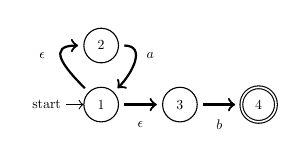
\begin{tikzpicture}
			[
				transform shape,
				scale=0.5,
				align=center,
				label/.style={draw=none,fill=none},
				arrow/.style={->, thick, shorten <=2pt, shorten >=2pt,}
			]

			% states
			\node[initial,state] (s1) at (  0.0,  0.0 ) {$1$};
			\node[state] (s2) at (  0.0,  1.5 ) {$2$};
			\node[state] (s3) at (  2.0,  0.0 ) {$3$};
			\node[state,accepting] (s4) at (  4.0,  0.0 ) {$4$};

			% transition labels
			\node[label] (s1s3) at (  1.0 , -0.5 ) {$\epsilon$};
			\node[label] (s3s4) at (  3.0 , -0.5 ) {$b$};
			\node[label] (s1s2) at ( -1.5 ,  1.25 ) {$\epsilon$};
			\node[label] (s2s1) at (  1.25,  1.25 ) {$a$};

			% transition paths
			\foreach \from/\to in {s1/s3,s3/s4}
			\draw[arrow] (\from) -> (\to);

			\draw[arrow] (s1) to [out=135,in=180,looseness=2] (s2);
			\draw[arrow] (s2) to [out=0,in=45,looseness=1.5] (s1);

		\end{tikzpicture}
		\label{fig:nfa-alpha-2}
		\caption{NFA for $\alpha_2$}
	\end{figure}

	\vfill
	\columnbreak

	\begin{figure}[H]
		\center
		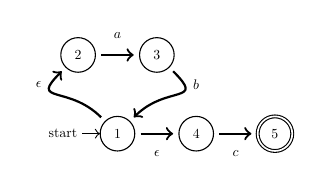
\begin{tikzpicture}
			[
				transform shape,
				scale=0.5,
				align=center,
				label/.style={draw=none,fill=none},
				arrow/.style={->, thick, shorten <=2pt, shorten >=2pt,}
			]

			% states
			\node[initial,state] (s1) at (  0.0,  0.0 ) {$1$};
			\node[state] (s2) at ( -1.0,  2.0 ) {$2$};
			\node[state] (s3) at (  1.0,  2.0 ) {$3$};
			\node[state] (s4) at (  2.0,  0.0 ) {$4$};
			\node[state,accepting] (s5) at (  4.0,  0.0 ) {$5$};

			% transition labels
			\node[label] (s1s2) at ( -2.0 ,  1.25 ) {$\epsilon$};
			\node[label] (s1s4) at (  1.0 , -0.5 ) {$\epsilon$};
			\node[label] (s2s3) at (  0.0 ,  2.5 ) {$a$};
			\node[label] (s3s1) at (  2.0 ,  1.25 ) {$b$};
			\node[label] (s4s5) at (  3.0 , -0.5 ) {$c$};

			% transition paths
			\foreach \from/\to in {s1/s4,s2/s3,s4/s5}
			\draw[arrow] (\from) -> (\to);

			\draw[arrow] (s1) to [out=135,in=225,looseness=2.0] (s2);
			\draw[arrow] (s3) to [out=315,in=45,looseness=2.0] (s1);

		\end{tikzpicture}
		\label{fig:nfa-alpha-3}
		\caption{NFA for $\alpha_3$}
	\end{figure}

\end{multicols}
And, yet again, following the rules for fragments, we combined these into a
non-deterministic finite automaton
\begin{figure}[H]
	\center
	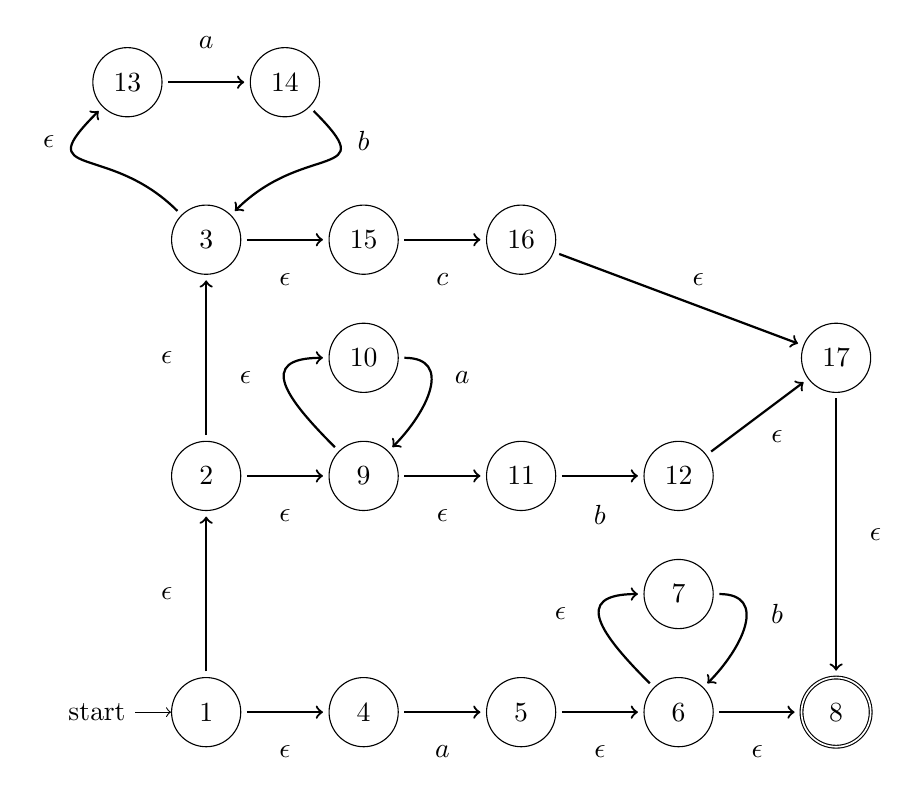
\begin{tikzpicture}
		[
			transform shape,
			align=center,
			label/.style={draw=none,fill=none},
			arrow/.style={->, thick, shorten <=2pt, shorten >=2pt,}
		]

		% states
		\node[initial left,state]	(s1) at (  0.0,  0.0 ) {$1$};
		\node[state]				(s17) at (  8.0,  4.5 ) {$17$};
		\node[state]				(s2) at (  0.0,  3.0 ) {$2$};
		\node[state]				(s3) at (  0.0,  6.0 ) {$3$};

		% transition labels
		\node[label] (s1s2)		at ( -0.5 ,  1.5 ) {$\epsilon$};
		\node[label] (s2s3)		at ( -0.5 ,  4.5 ) {$\epsilon$};

		% transition paths
		\foreach \from/\to in {s1/s2,s2/s3}
		\draw[arrow] (\from) -> (\to);

		% states for alpha one
		\node[state] (s4) at (  2.0,  0.0 ) {$4$};
		\node[state] (s5) at (  4.0,  0.0 ) {$5$};
		\node[state] (s6) at (  6.0,  0.0 ) {$6$};
		\node[state] (s7) at (  6.0,  1.5 ) {$7$};
		\node[state,accepting] (s8) at (  8.0,  0.0 ) {$8$};

		% transition labels for alpha one
		\node[label] (s1s4) at (  1.0 , -0.5 ) {$\epsilon$};
		\node[label] (s4s5) at (  3.0 , -0.5 ) {$a$};
		\node[label] (s5s6) at (  5.0 , -0.5 ) {$\epsilon$};
		\node[label] (s6s8) at (  7.0 , -0.5 ) {$\epsilon$};
		\node[label] (s6s7) at (  4.5 ,  1.25 ) {$\epsilon$};
		\node[label] (s7s6) at (  7.25,  1.25 ) {$b$};

		% transition paths for alpha one
		\foreach \from/\to in {s1/s4,s4/s5,s5/s6,s6/s8}
		\draw[arrow] (\from) -> (\to);

		\draw[arrow] (s6) to [out=135,in=180,looseness=2] (s7);
		\draw[arrow] (s7) to [out=0,in=45,looseness=1.5] (s6);

		% states for alpha two
		\node[state] (s9) at (  2.0,  3.0 ) {$9$};
		\node[state] (s10) at (  2.0,  4.5 ) {$10$};
		\node[state] (s11) at (  4.0,  3.0 ) {$11$};
		\node[state] (s12) at (  6.0,  3.0 ) {$12$};

		% transition labels for alpha two
		\node[label] (s2s9) at (  1.0 ,  2.5 ) {$\epsilon$};
		\node[label] (s9s11) at (  3.0 ,  2.5 ) {$\epsilon$};
		\node[label] (s11s12) at (  5.0 , 2.5 ) {$b$};
		\node[label] (s2s10) at (  0.5 ,  4.25 ) {$\epsilon$};
		\node[label] (s10s2) at (  3.25,  4.25 ) {$a$};

		% transition paths for alpha two
		\foreach \from/\to in {s2/s9,s9/s11,s11/s12}
		\draw[arrow] (\from) -> (\to);

		\draw[arrow] (s9) to [out=135,in=180,looseness=2] (s10);
		\draw[arrow] (s10) to [out=0,in=45,looseness=1.5] (s9);

		% states for alpha three
		\node[state] (s13) at ( -1.0,  8.0 ) {$13$};
		\node[state] (s14) at (  1.0,  8.0 ) {$14$};
		\node[state] (s15) at (  2.0,  6.0 ) {$15$};
		\node[state] (s16) at (  4.0,  6.0 ) {$16$};

		% transition labels for alpha three
		\node[label] (s3s13) at ( -2.0 ,  7.25 ) {$\epsilon$};
		\node[label] (s3s15) at (  1.0 ,  5.5 ) {$\epsilon$};
		\node[label] (s13s14) at (  0.0 ,  8.5 ) {$a$};
		\node[label] (s14s3) at (  2.0 ,  7.25 ) {$b$};
		\node[label] (s15s16) at (  3.0 , 5.5 ) {$c$};

		% transition paths for alpha three
		\foreach \from/\to in {s3/s15,s13/s14,s15/s16}
		\draw[arrow] (\from) -> (\to);

		\draw[arrow] (s3) to [out=135,in=225,looseness=2.0] (s13);
		\draw[arrow] (s14) to [out=315,in=45,looseness=2.0] (s3);

		% fragment transition labels
		\node[label] (s16s17)	at ( 6.25,  5.50 ) {$\epsilon$};
		\node[label] (s12s17)	at ( 7.25,  3.50 ) {$\epsilon$};
		\node[label] (s17s8)	at ( 8.50,  2.25 ) {$\epsilon$};

		% fragment transition paths
		\foreach \from/\to in {s16/s17,s12/s17,s17/s8}
		\draw[arrow] (\from) -> (\to);

	\end{tikzpicture}
	\label{fig:nfa-combined}
	\caption{The combined NFA for $\alpha_1$, $\alpha_2$ and $\alpha_3$}
\end{figure}
The figure above shows the non-deterministic finite automaton which we arrive
at.
\newpage
\subsection*{b \mdseries Convert this combined NFA to a DFA by subset
construction.}
Now that we have a non-deterministic finite automaton for the languages
$L(\alpha_1)$, $L(\alpha_2)$ and $L(\alpha_3)$, we can convert this to a
deterministic finite automaton by subset construction.
\vspace{-0.25in}
\begin{multicols}{2}
	\begin{align*}
		E &= \hat{\epsilon}(\emptyset) = \emptyset \not\subset F \\
		S_0 &= \hat{\epsilon}(\{1\}) = \{1,2,3,4,9,10,11,13,15\} \\
		S_1 &= \hat{\epsilon}(\{5,9,14\}) = \{5,6,7,8,9,10,11,13,14\} \subset F \\
		S_2 &= \hat{\epsilon}(\{5\}) = \{5,6,7,8\} \subset F \\
		S_3 &= \hat{\epsilon}(\{9\}) = \{9,10,11\} \not\subset F
	\end{align*}
	\vfill
	\columnbreak
	\begin{align*}
		S_4 &= \hat{\epsilon}(\{14\}) = \{14\} \not\subset F \\
		S_5 &= \hat{\epsilon}(\{3\}) = \{3,13\} \not\subset F \\
		S_6 &= \hat{\epsilon}(\{12\}) = \{8,12,17\} \subset F \\
		S_7 &= \hat{\epsilon}(\{6\}) = \{6,7,8\} \subset F \\
		S_8 &= \hat{\epsilon}(\{16\}) = \{8,16,17\} \subset F
	\end{align*}
	\vfill
\end{multicols}
From these $\epsilon$-closures, we can construct the deterministic finite
automaton.
\begin{figure}[H]
	\center
	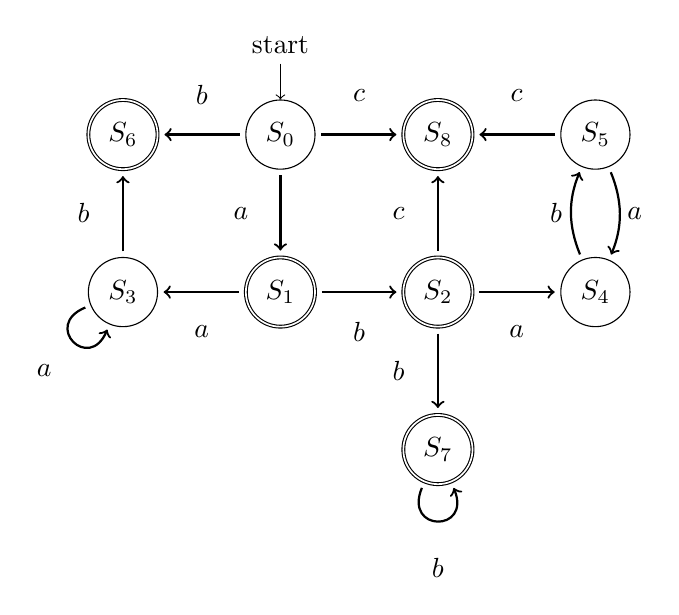
\begin{tikzpicture}
		[
			transform shape,
			scale=1.0,
			align=center,
			label/.style={draw=none,fill=none},
			arrow/.style={->, thick, shorten <=2pt, shorten >=2pt,}
		]

		% states
		\node[initial above,state]	(S0) at (  2.0,  2.0 ) {$S_0$};
		\node[state, accepting]		(S1) at (  2.0,  0.0 ) {$S_1$};
		\node[state, accepting]		(S2) at (  4.0,  0.0 ) {$S_2$};
		\node[state]				(S3) at (  0.0,  0.0 ) {$S_3$};
		\node[state]				(S4) at (  6.0,  0.0 ) {$S_4$};
		\node[state]				(S5) at (  6.0,  2.0 ) {$S_5$};
		\node[state, accepting]		(S6) at (  0.0,  2.0 ) {$S_6$};
		\node[state, accepting]		(S7) at (  4.0, -2.0 ) {$S_7$};
		\node[state, accepting]		(S8) at (  4.0,  2.0 ) {$S_8$};

		% transition labels
		\node[label] (A)			at (  1.50 ,  1.00 ) {$a$};
		\node[label] (AA)			at (  1.00 , -0.50 ) {$a$};
		\node[label] (A*)			at ( -1.00 , -1.00 ) {$a$};
		\node[label] (A*B)			at ( -0.50 ,  1.00 ) {$b$};
		\node[label] (AB)			at (  3.00 , -0.50 ) {$b$};
		\node[label] (ABB)			at (  3.50 , -1.00 ) {$b$};
		\node[label] (AB*)			at (  4.00 , -3.50 ) {$b$};
		\node[label] (ABC)			at (  3.50 ,  1.00 ) {$c$};
		\node[label] (B)			at (  1.00 ,  2.50 ) {$b$};
		\node[label] (C)			at (  3.00 ,  2.50 ) {$c$};
		\node[label] (ABA)			at (  5.00 , -0.50 ) {$a$};
		\node[label] (ABAB)			at (  5.50 ,  1.00 ) {$b$};
		\node[label] (AB*)			at (  6.50 ,  1.00 ) {$a$};
		\node[label] (AB*C)			at (  5.00 ,  2.50 ) {$c$};

		% transition paths
		\foreach \from/\to in
		{S0/S1,S0/S6,S0/S8,S1/S2,S1/S3,S2/S4,S5/S8,S2/S7,S2/S8,S3/S6}
		\draw[arrow] (\from) -> (\to);

		\draw[arrow] (S3) to [out=202.5,in=247.5,looseness=5] (S3);
		\draw[arrow] (S4) to [out=112.5,in=247.5,looseness=1.0] (S5);
		\draw[arrow] (S5) to [out=292.5,in=67.5,looseness=1.0] (S4);
		\draw[arrow] (S7) to [out=247.5,in=292.5,looseness=5] (S7);

	\end{tikzpicture}
	\label{fig:dfa-subset-construction}
	\caption{Subset constructed NFA for the languages $L(\alpha_1)$,
	$L(\alpha_2)$ and $L(\alpha_3)$}
\end{figure}
And this is the final deterministic finite automaton.

% α1: ab*
% α2: a*b
% α3: (ab)*c

\subsection*{c \mdseries Describe the transitions and backtracking steps used
when the combined DFA analyses the input {\tt "ababacca"}.}
\begin{figure}[H]
	\center
	\begin{tabular}{|c|c|c|c|c|c|}
		\hline
		{\bf \#} & {\bf State} & {\bf Tokens} & {\bf Matches} & {\bf Analyzed} & {\bf Buffer} \\ \hline
		$0$ & $S_0$ & $\emptyset$ & $\emptyset$ & {\tt ""} & {\tt "ababacca"}
		\\ \hline
		$1$ & $S_1$ & $\emptyset$ & $\{\alpha_1\}$ & {\tt "a"} & {\tt "babacca"}
		\\ \hline
		$2$ & $S_2$ & $\emptyset$ & $\{\alpha_1,\alpha_2\}$ & {\tt "ab"} & {\tt "abacca"}
		\\ \hline
		$3$ & $S_4$ & $\emptyset$ & $\emptyset$ & {\tt "aba"} & {\tt "bacca"}
		\\ \hline
		$4$ & $S_5$ & $\emptyset$ & $\emptyset$ & {\tt "abab"} & {\tt "acca"}
		\\ \hline
		$5$ & $S_4$ & $\emptyset$ & $\emptyset$ & {\tt "ababa"} & {\tt "cca"}
		\\ \hline
		$6$ & $S_2$ & $\emptyset$ & $\{\alpha_1,\alpha_2\}$ & {\tt "ab"} & {\tt "abacca"}
		\\ \hline
		$7$ & $S_0$ & $\{\alpha_1\}$ & $\emptyset$ & {\tt ""} & {\tt "abacca"}
		\\ \hline
		\vdots & \vdots & \vdots & \vdots & \vdots & \vdots
		\\ \hline
		$8$ & $S_0$ & $\{\alpha_1,\alpha_1\}$ & $\emptyset$ & {\tt ""} & {\tt "acca"}
		\\ \hline
		$9$ & $S_1$ & $\{\alpha_1,\alpha_1\}$ & $\{\alpha_1,\alpha_2\}$ & {\tt "a"} & {\tt "cca"}
		\\ \hline
		$10$ & N/A & $\{\alpha_1,\alpha_1\}$ & $\emptyset$ & {\tt "ac"} & {\tt "ca"}
		\\ \hline
		$11$ & $S_0$ & $\{\alpha_1,\alpha_1,\alpha_1\}$ & $\emptyset$ & {\tt ""} & {\tt "cca"}
		\\ \hline
		$12$ & $S_8$ & $\{\alpha_1,\alpha_1,\alpha_1\}$ & $\{\alpha_3\}$ & {\tt "c"} & {\tt "ca"}
		\\ \hline
		$13$ & N/A & $\{\alpha_1,\alpha_1,\alpha_1\}$ & $\emptyset$ & {\tt "cc"} & {\tt "a"}
		\\ \hline
		$14$ & $S_0$ & $\{\alpha_1,\alpha_1,\alpha_1,\alpha_3\}$ & $\emptyset$ & {\tt ""} & {\tt "ca"}
		\\ \hline
		$15$ & $S_8$ & $\{\alpha_1,\alpha_1,\alpha_1,\alpha_3\}$ & $\{\alpha_3\}$ & {\tt "c"} & {\tt "a"}
		\\ \hline
		$16$ & N/A & $\{\alpha_1,\alpha_1,\alpha_1,\alpha_3\}$ & $\emptyset$ & {\tt "ca"} & {\tt ""}
		\\ \hline
		$17$ & $S_0$ & $\{\alpha_1,\alpha_1,\alpha_1,\alpha_3,\alpha_3\}$ & $\emptyset$ & {\tt ""} & {\tt "a"}
		\\ \hline
		$18$ & $S_1$ & $\{\alpha_1,\alpha_1,\alpha_1,\alpha_3,\alpha_3\}$ & $\{\alpha_1\}$ & {\tt "a"} & {\tt ""}
		\\ \hline
		$18$ & $S_1$ & $\{\alpha_1,\alpha_1,\alpha_1,\alpha_3,\alpha_3,\alpha_1\}$ & $\emptyset$ & {\tt ""} & {\tt EOF}
		\\ \hline
	\end{tabular}
	\label{table:backtracking}
	\caption{Analyzing the string {\tt "ababacca"} using the DFA}
\end{figure}
Having done the analysis of the string through the DFA we have built, we get
the token set $\{\alpha_1,\alpha_1,\alpha_1,\alpha_3,\alpha_3,\alpha_1\}$,
which corresponds to what we would expect, given that $\alpha_1$ has been
given higher priority than $\alpha_2$.

\newpage
\section{Mosmllex Scanner Construction}
Use Mosmllex to implement a scanner for the regular expressions $\alpha_1$,
$\alpha_2$, and $\alpha_3$ from task 1.2. Use the generated scanner to verify
your solution of part 1.2 (c).
\lstinputlisting[language=ML]{scanner.lex}
For the raw code please see attached file {\tt scanner.lex}. In order to
generate the scanner, issue the command {\tt mosmllex scanner.lex} and to test
the solution {\tt mosml script.sml}.
\\\\
The verification was done by running {\tt mosml script.sml} and issuing
{\tt Scan "ababacca";} in interactive mode, and came back with the expected
result:\\
{\tt [AlphaOne "ab", AlphaOne "ab", AlphaOne "ab",\\AlphaThree "c", AlphaThree
"c", AlphaOne "a"]}

\section{More on Regular Languages and Tokenisation}

\subsection*{a \mdseries Using the alphabet of decimal digits, give regular
expression describing the following languages:}
\begin{enumerate}[i]
	\item Numbers divisible by 5.\\
	\verb/([1-9]+(0|5))|5/
	\item Numbers in which digit '5' occurs exactly three times.\\
	Under the assumption that there shouldn't be any zeros in front.\\
	\verb/([1-9][0-9]*)?5[0-9]*5[0-9]*5[0-9]*/
\end{enumerate}

\subsection*{b \mdseries Are the following languages over the alphabet of
decimal digits regular? Give short convincing reasons for your answers.}
\begin{enumerate}[i]
	\item Numbers which contain digit '1' exactly as many times as digit '2'.\\
	No, as it is impossible to write a recursive regular expression, or form a
	finite automaton with this property.
	\item Numbers $N < 1.000.000$ which contain digit '1' exactly as often as
	digit '2'.\\
	Although tedious to define, this is a finite set of strings over the
	alphabet, and as such is indeed regular.
\end{enumerate}

\end{document}
